\section{Electronics}


%Semiconductors (PN junction)


%Diodes

\subsection{Forward and Reverse Biased Diodes}

\subsubsection*{Learning Objectives}
\begin{itemize}
\item{To explain the mode of action of a P-N junction} 
\end{itemize}

\subsubsection*{Background Information}
An extrinsic semiconductor has a net positive or negative charge. For example, silicon doped with phosphorus has a negative charge and is called an N-Type semiconductor. Silicon doped with boron has a positive charge and is called a P-Type semiconductor. When these two types of semiconductors are connected in series, they form a P-N Junction.  
We know that electric current flows from positive to negative in a circuit.  

\subsubsection*{Materials}
Diode, dry cell, bulb, connecting wires, nail, heat source or soldering iron

\subsubsection*{Preparation Procedure}
\begin{enumerate}
\item{Heat the soldering iron or nail.}
\item{Remove a diode from broken radio using a soldering iron or a hot nail.} 
\end{enumerate}

\subsubsection*{Activity Procedure}
\begin{enumerate}
\item{Join the bulb in series with the P-N junction.} 
\item{Connect the P-terminal of the junction to the positive pole dry cell and the N-terminal of the junction to the negative pole of the dry cell.} 
\item{Record what you observe in the circuit.} 
\item{Reverse the terminal of the cell and observe the change in the circuit.} 
\end{enumerate}

\begin{figure}
\begin{center}
%\def\svgwidth{250pt}
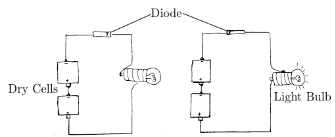
\includegraphics{./img/diode.png}
\caption{Testing the Action of a Diode}
\label{fig:diode}
\end{center}
\end{figure}

\subsubsection*{Results and Conclusions}
When the P-terminal of the junction (diode) is connected to the positive terminal of the battery and the N-terminal of the junction is connected to the negative terminal of the battery, the bulb will light, indicating that current is flowing.  
If the terminals are reversed so that the P-terminal is connected to the negative battery terminal and the N-terminal is connected to the positive battery terminal, the bulb will not light, indicating that current is not flowing.  
The P-N junction, allows current to flow only in one direction; current can flow from the P-terminal to the N-terminal, but not the other way.  
Current always flows from a positive terminal to a negative terminal.  

\subsubsection*{Clean Up Procedure}
Disconnect the apparatus and return materials to their proper place.

\subsubsection*{Discussion Questions}
\begin{enumerate}
\item{What is a diode?}
\item{What will happen when the P-terminal of the junction is connected to the negative pole of the cell?}
\item{Why does a diode allow current to flow in only one direction?}
\end{enumerate}

\subsubsection*{Notes}
A diode, which can be found in a radio, phone charger, etc.  , has two colours: white and black. The black side is the P-terminal and the white band is the N-terminal. Current will only flow from the black side to the white side.  

	%Half-wave, full-wave rectifiers
	
\subsection{Full-Wave Rectifier}

\subsubsection*{Learning Objectives}
\begin{itemize}
\item{To observe the effects of full-wave rectification on a galvanometer and bulb}
\item{To explain the mode of action of a full-wave rectifier}
\item{To explain the use of diodes in a full-wave rectifier}
\item{To explain the relationship between AC current, full-wave rectification and half-wave rectification}
\end{itemize}

\subsubsection*{Background Information}
AC is current which changes direction many times per second.  When we want to change AC to DC, which moves in only one direction, we must use a wave-rectifier.  A half-wave rectifier is simple to make and use, but it only converts half of the AC current to DC.  In order to convert more AC current to DC, we need to use a full-wave rectifier.
A full-wave rectifier allows current in one direction to pass.  It then takes current in the opposite direction and changes its direction so that it can pass again.  For example, all forward-moving current will pass a wave rectifier.  Then all current which is moving backward will have its direction changed so that it can pass the rectifier.  In this way, all of the AC current is used and changed to DC.

\subsubsection*{Materials}
Low voltage AC power source (see the activity "Inverter"), connecting wires, 4 diodes, bulb, resistor, galvanometer, optional super glue

\subsubsection*{Hazards and Safety}
\begin{itemize}
\item{Do not use the power from outlets in a house or school.  These outlets put out a high voltage (220 V) which can kill you.  Instead use a laboratory power supply or use D-cell batteries with an inverter as described above.}
\end{itemize}

\subsubsection*{Preparation Procedure}
\begin{enumerate}
\item{Collect all materials.}
\item{Connect the AC power supply to the galvanometer to make sure that it is working.  If you don't have an AC power supply in your school, you can create an inverter which converts the DC output of a battery into AC.  This process is described in the "Inverter" activity.}
\item{Connect two diodes together in series with connecting wire.  Use super glue to help secure them if you do not have a breadboard.}
\item{Repeat this step so that you have two pairs of diodes in series.}
\item{Connect these pairs in parallel to each other so that current can flow through either pair but only in one direction.}
\item{Also connect a resistor and a galvanometer in parallel across the pairs of diodes.  Now you should have four things in parallel: two pairs of diodes with the same direction, a galvanometer and a resistor.}
\item{Attach connecting wires between the diodes in each pair.}
\item{Extend these connecting wires to the AC power source.  Now the AC power source should be attached to the middle of each diode pair.}
\item{Attach a bulb in parallel across the AC source.}
\end{enumerate}

\begin{figure}
\begin{center}
%\def\svgwidth{250pt}
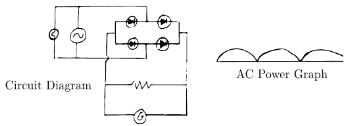
\includegraphics{./img/full-wave-rectifier.png}
\caption{Full Wave Rectifier}
\label{fig:full-wave-rectifier}
\end{center}
\end{figure}

\subsubsection*{Activity Procedure}
\begin{enumerate}
\item{Test the AC power source to see that the bulb flickers.}
\item{Connect the AC source directly to the galvanometer and observe the behavior of the galvanometer.}
\item{Connect the AC source to the full-wave rectifier and observe the behavior of the galvanometer in relation to the bulb.}
\end{enumerate}

\subsubsection*{Results and Conclusions}
When the AC source is connected directly to the galvanometer, the galvanometer needle will jump one direction and then the other, showing the changing direction of current through the circuit.  However, when the galvanometer is powered through the full-wave rectifier, it can be seen that the galvanometer only indicates one direction (positive or negative) and jumps quickly between zero and its maximum value.

If observed closely with an AC source of low frequency, it can be seen that the bulb and galvanometer flicker at exactly the same rate.  This is because the full-wave rectifier creates DC current which increases and decreases (but only in one direction) at the same frequency that the AC current is changing direction.  As the bulb is following the AC current at a certain frequency, the galvanometer is being driven by the DC current at the same frequency of increasing and decreasing.

\subsubsection*{Clean Up Procedure}
\begin{enumerate}
\item{Turn off the power supply and disconnect the wires.}
\item{Return all materials to their proper places.}
\end{enumerate}

\subsubsection*{Discussion Questions}
\begin{enumerate}
\item{What is the behavior of the galvanometer when connected directly to the AC source?}
\item{What is the behavior of the galvanometer when connected to the full-wave rectifier?}
\item{Compare the behavior of the galvanometer and the bulb when the galvanometer is connected to the full-wave rectifier and the bulb is connected to the AC source.}
\end{enumerate}

\subsubsection*{Notes}
This activity is normally done with an oscilloscope, which clearly shows the waveform of the AC current and rectified current.  However, the effect of the full-wave rectifier can be seen clearly if you are using the correct components.

First, the full-wave rectification can be compared to the half-wave rectification.  If you connect the AC source to both a half-wave rectifier and a full-wave rectifier, each with a galvanometer, it can be seen that the full-wave rectifier causes the galvanometer to move at twice the speed of the half-wave rectifier.

Also, when a bulb is attached in parallel across the AC source while the galvanometer reads the current through the full-wave rectifier, it can be seen that the bulb and galvanometer flicker at the same rate, proving that the entire AC wave is being converted directly to DC rather than only half of the wave.

\subsection{Half-Wave Rectifier}

\subsubsection*{Learning Objectives}
\begin{itemize}
\item{To observe the effects of half-wave rectification on alternating current}
\item{To construct a half-wave rectifier}
\item{To explain the mode of action of a half-wave rectifier}
\item{To explain the use of a diode}
\end{itemize}

\subsubsection*{Background Information}
Alternating current is current which changes direction many times per second.  It is useful for transporting electric current over great distances but it is not always useful in appliances in the home or school.  For this reason, we often need to convert alternating current into direct current, which moves only in one direction.

One way to do this is to make a one-way gate through which electric current can pass in one direction but not in another.  A device which does this easily is a diode, or P-N Junction, which allows current to pass from the P-type to the N-type semiconductor of the diode.  By passing AC through a diode, we produce direct current whenever the AC is moving forward, and no current whenever the AC is moving backward.  The result is a half-wave of electric current, where we recover (or rectify) half of the AC current and convert it into DC.

\subsubsection*{Materials}
Low power AC power source (see the activity "Inverter"), diode, bulb, galvanometer, connecting wires.

\subsubsection*{Hazards and Safety}
\begin{itemize}
\item{Do not use the AC power of an outlet in your home or school.  These outlets carry very high voltage (220 V) which can kill you if you are not careful.  Instead, use a low-power AC power supply.}
\end{itemize}

\subsubsection*{Preparation Procedure}
\begin{enumerate}
\item{Collect all materials.}
\item{If you don't have an AC power supply, you can construct an inverter which converts the DC of batteries into AC.}
\item{Set up the power source or inverter to produce AC current and check that it is AC by watching its effect on a galvanometer.}
\item{Connect the P-side of a diode (the black colour indicates P-type) to one of the connecting wires from the power source.}
\item{Connect one of the terminals of the bulb to the N-side of the diode (a white band indicates N-type).}
\item{Connect the other terminal of the bulb to the remaining connecting wire of the power source.  You should now have a power source, diode and bulb all in series.}
\item{Connect the galvanometer in parallel with the bulb.}
\end{enumerate}

\begin{figure}
\begin{center}
\def\svgwidth{180pt}
\input{./img/half-wave-rectifier.pdf_tex}
\caption{Half Wave Rectifier}
\label{fig:half-wave-rectifier}
\end{center}
\end{figure}

\subsubsection*{Activity Procedure}
\begin{enumerate}
\item{Turn on the power and watch the behavior of the galvanometer.}
\end{enumerate}

\subsubsection*{Results and Conclusions}
When AC power is connected to a galvanometer, it is seen that the current is changing direction quickly, causing the needle to jump back and forth.  When the AC is passed through a half-wave rectifier, however, the current is only in one direction (positive or negative) and jumps between zero and the maximum value at half the speed that it did with AC current.
This is because the AC current is being cut in half through the rectifier and is allowed to move in only one direction.  If using a bulb, it will be seen that the bulb flickers quickly with AC current, but only half as quickly with half-wave rectified current.

\subsubsection*{Clean Up Procedure}
\begin{enumerate}
\item{Disconnect all wires and turn off the power supply.}
\item{Return all materials to their proper places.}
\end{enumerate}

\subsubsection*{Discussion Questions}
\begin{enumerate}
\item{What is the difference shown by the galvanometer between regular AC current and AC current when it is passed through the half-wave rectifier?}
\item{Is the speed of the galvanometer needle the same in both cases, or different?}
\end{enumerate}

\subsubsection*{Notes}
This activity is normally done with an oscilloscope, which shows the wave pattern of the AC current (it is a sine wave).  If seen on the oscilloscope, the AC appears as a full sine wave, while the half-wave rectified current appears as only the positive or negative part of the sine wave (it looks like hills separated by long spaces).
A half-wave rectifier, rather than converting AC directly to DC, simply removes all current in one direction and allows all current in the other direction.  In this way, the product is direct current, but only half of what was produced by the AC power source.


%Transistors (npn, pnp)


%Electronic Amplifiers

